\documentclass{beamer}

\usepackage{moy-slides}
\usepackage{tikz}
\usepackage{comment}
\usepackage{listings}

\title[Path-focusing]{Using bounded model checking to focus fixpoint iterations}

%\subtitle{} % (optional)

\author[Julien Henry]{Julien Henry}
% - Use the \inst{?} command only if the authors have different
%   affiliation.

\institute[Verimag]{Verimag (Grenoble INP)\\Grenoble\\France}

\tikzstyle{arrow}=[->,line width=.05cm,draw=red!90!blue!60!black]

\usetikzlibrary{snakes,arrows,shapes,backgrounds,shadows,automata,patterns}
\usepgflibrary{snakes}

\tikzstyle{state}=[circle,fill=black!25,minimum size=13pt,inner sep=0pt]
\tikzstyle{transition}=[rectangle,thick,draw=black!75,
  			  fill=black!20,minimum size=4mm]
\tikzstyle{transition2}=[rectangle,thick,draw=blue!75,
  			  fill=blue!20,minimum size=4mm,blue]
\tikzstyle{PRstate}=[circle,fill=red!90,minimum size=13pt,inner sep=0pt]
\tikzstyle{polyhedra}=[blue!25,opacity=0.5,pattern=north west lines,pattern
color=blue]
\tikzstyle{line}=[black,thick]

\date{March 22$^{th}$ 2011}

\begin{document}

\begin{frame}
  \titlepage
\end{frame}

\begin{frame}[containsverbatim]
\frametitle{Abstract Interpretation}
$x \in [0,1]$

$y \in [0,1]$

\begin{lstlisting}
z = x+y;
x = z-y;
\end{lstlisting}
\end{frame}

\begin{frame}
\frametitle{Sources of imprecision}
\begin{itemize}
\item transformation that can't be expressed in the abstract domain
\item widening operator
\item consider paths that can't be taken in reality
\end{itemize}
\end{frame}

\begin{frame}
  \frametitle{Introduction}
\begin{itemize}
\item Abstract interpretation.
\item Widening operator:
\begin{itemize}
\item ensure fast convergence
\item BUT: may induce huge imprecisions
\end{itemize}
\end{itemize}
\end{frame}

\begin{frame}
\frametitle{Summary}
\tableofcontents
\end{frame}

\section[Introduction]{Introduction: Weakness of the standard approach}


\begin{frame}[containsverbatim]
  \frametitle{Example of standard Abstract Interpretation}
\begin{center}
\begin{lstlisting}
	x = 0;
	y = 0;
	while (true) {
		if (x <= 50) y++;
		else y--;
	
		if (y < 0) break;
		x++;
	}
\end{lstlisting}
\end{center}

\begin{itemize}
\item  $x$ and $y$ incremented during 51 iterations
\item  $x$ incremented and $y$ decremented during 51 iterations
\end{itemize}

\end{frame}

\begin{frame}
  \frametitle{Example of standard Abstract Interpretation}

\begin{columns}
  \begin{column}{6cm}
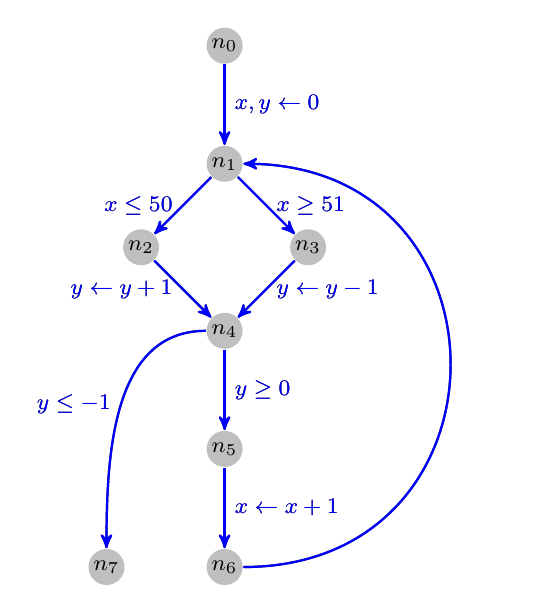
\begin{tikzpicture}[->,>=stealth',auto,node distance=1.5cm,
                    semithick,font=\footnotesize]

	\node[state] (n0) {$n_0$};
	\node[state] (n1) [below of=n0] {$n_1$};
	\node[state] (n2) [below left of=n1] {$n_2$};
	\node[state] (n3) [below right of=n1] {$n_3$};
	\node[state] (n4) [below left of=n3] {$n_4$};
	\node[state] (n5) [below of=n4] {$n_5$};
	\node[state] (n6) [below of=n5] {$n_6$};
	\node[state] (n7) [left of=n6] {$n_7$};

	\node (n8) [right of=n6] {};
	\node (n9) [right of=n1] {};

  \path<-1> [transition] 
		(n0) edge              node {$x,y \leftarrow 0$} (n1);
  \path<-2> [transition] 
        (n1) edge			   node [left] {$x \leq 50$} (n2);
  \path<-8> [transition] 
        (n1)  edge              node [right] {$x \geq 51$} (n3);
  \path<-3> [transition] 
        (n2) edge              node [left] {$y \leftarrow y+1$} (n4);
  \path<-9> [transition] 
        (n3) edge			   node [right] {$y \leftarrow y-1$} (n4);
  \path<-4> [transition] 
        (n4) edge			   node {$y \geq 0$} (n5);
  \path<-11> [transition] 
		(n4) edge  [out = 180, in=90] node [left] {$y \leq -1$} (n7);
  \path<-5> [transition] 
        (n5) edge              node {$x \leftarrow x+1$} (n6);
  \path<-6> [transition] 
        (n6) edge [out=0, in=0, distance=3.5cm] node {} (n1);

  \path<2-> [transition2] 
		(n0) edge              node {$x,y \leftarrow 0$} (n1);
  \path<3-> [transition2] 
        (n1) edge			   node [left] {$x \leq 50$} (n2);
  \path<9-> [transition2] 
        (n1)  edge              node [right] {$x \geq 51$} (n3);
  \path<4-> [transition2] 
        (n2) edge              node [left] {$y \leftarrow y+1$} (n4);
  \path<10-> [transition2] 
        (n3) edge			   node [right] {$y \leftarrow y-1$} (n4);
  \path<5-> [transition2] 
        (n4) edge			   node {$y \geq 0$} (n5);
  \path<12-> [transition2] 
		(n4) edge  [out = 180, in=90] node [left] {$y \leq -1$} (n7);
  \path<6-> [transition2] 
        (n5) edge              node {$x \leftarrow x+1$} (n6);
  \path<7-> [transition2] 
        (n6) edge [out=0, in=0, distance=3.5cm] node {} (n1);
\end{tikzpicture}
\end{column}
\begin{column}{5cm}
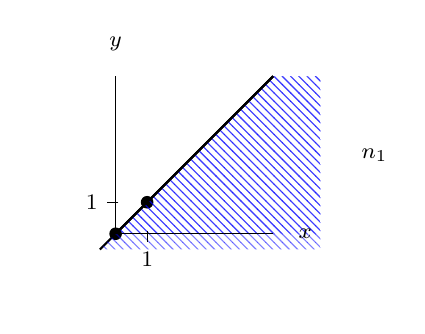
\begin{tikzpicture}[y=.2cm, x=.2cm,font=\footnotesize]

	\node (t1) at (-5,-4) {};
	\node (t2) at (13,11) {};
	\fill<2-7>[line] (0,0) circle (0.4);
	\fill<7>[line] (2,2) circle (0.4);
	\draw<8-10>[line] (0,0) -- (10,10) -- cycle;
	\draw<11-12>[line] (-1,-1) -- (10,10) -- cycle;
	\fill<11-12>[polyhedra] (-1,-1) -- (10,10) -- (13,10) -- (13,-1) -- (0,-1) -- cycle;
	\fill<13-14>[polyhedra] (0,0) -- (10,10) -- (13,10) -- (13,0) -- cycle;
	\draw<13-14>[line] (0,0) -- (10,10) -- cycle;

 	%axis
	\draw (0,0) -- coordinate (x axis mid) (10,0);
    \draw (0,0) -- coordinate (y axis mid) (0,10);

	%ticks and labels      
	\node[right=1.2cm] at (x axis mid) {$x$};
	\node[above=1.2cm] at (y axis mid) {$y$};

	\node[right=3cm] at (y axis mid) {$n_1$};

    \draw<7> (1pt,2) -- (-3pt,2) 
     	node[anchor=east] {1}; 
    \draw<7> (2,1pt) -- (2,-3pt) 
     	node[anchor=north] {1}; 

\end{tikzpicture} 
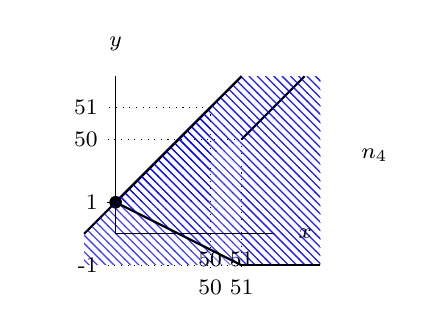
\begin{tikzpicture}[y=.2cm, x=.2cm,font=\footnotesize]

	\node (t1) at (-5,-4) {};
	\node (t2) at (13,11) {};
	\fill<4-9>[line] (0,2) circle (0.4);
	\fill<10-11>[polyhedra] (0,2) -- (8,10) -- (12,10) -- (8,6) --cycle;
	\draw<10-11>[line] (0,2) -- (6,8);
	\draw<10-11>[line] (8,6) -- (12,10);

	\draw<12-13>[line] (-2,0) -- (8,10);
	\fill<12-13>[polyhedra] (-2,-2) -- (-2,0) -- (8,10) -- (13,10) -- (13,-2) --
	 cycle;
	\fill<12-13>[polyhedra] (-2,-2) -- (-2,0) -- (6,8) -- (6,-2) -- cycle;
	\fill<12-14>[polyhedra] (8,6) -- (12,10) -- (13,10) -- (13,-2) -- (8,-2) -- cycle;

	\draw<14>[line] (0,2) -- (8,10);
	\draw<14>[line] (0,2) -- (8,-2);
	\draw<14>[line] (13,-2) -- (8,-2);
	\fill<14>[polyhedra] (0,2) -- (8,10) -- (13,10) -- (13,-2) -- (8,-2) -- cycle;
	\fill<14>[polyhedra] (0,2) -- (6,8) -- (6,2) --  cycle;

 	%axis
	\draw (0,0) -- coordinate (x axis mid) (10,0);
    \draw (0,0) -- coordinate (y axis mid) (0,10);

	%labels      
	\node[right=1.2cm] at (x axis mid) {$x$};
	\node[above=1.2cm] at (y axis mid) {$y$};

	\node[right=3cm] at (y axis mid) {$n_4$};
	%ticks
     		\draw<4-> (1pt,2) -- (-3pt,2) 
     			node[anchor=east] {1}; 
     		\draw<14-> [dotted](8,-2) -- (-3pt,-2) 
     			node[anchor=east] {-1}; 
	
     		\draw<10-> [dotted](6,8) -- (-3pt,8) 
     			node[anchor=east] {$51$}; 
     		\draw<10-> [dotted] (8,6) -- (-3pt,6) 
     			node[anchor=east] {$50$}; 
     		\draw<10-11> [dotted](8,6) -- (8,-3pt) 
     			node[anchor=north] {$51$}; 
     		\draw<10-11> [dotted] (6,8) -- (6,-3pt) 
     			node[anchor=north] {$50$}; 
     		\draw<12-> [dotted](8,6) -- (8,-2.3) 
     			node[anchor=north] {$51$}; 
     		\draw<12-> [dotted] (6,8) -- (6,-2.3) 
     			node[anchor=north] {$50$}; 
     		%\draw (2,1pt) -- (2,-3pt) 
     		%	node[anchor=north] {1}; 

\end{tikzpicture} 
\only<1-11>{Ascending iterations}
\only<12-13>{Descending iterations}
\end{column}
\end{columns}
\end{frame}

\begin{frame}
  \frametitle{Weakness of this approach}
	\begin{center}
		yields imprecision when a loop has several phases.
	\end{center}
\end{frame}

\begin{frame}
  \frametitle{My work}
\begin{enumerate}
\item Trying new methods to improve precision of the analysis.
\item Implementation of these methods, using:
\begin{itemize}
\item LLVM (Low Level Virtual Machine)
\item Apron library
\item SMT-solvers like Yices, Z3\ldots
\end{itemize}
\item Make some experiments and trying to solve shotcomings.
\end{enumerate}
\end{frame}

\section[Lookahead Widening]{Lookahead Widening method}

\begin{frame}
  \frametitle{Principle}

D. Gopan \& T. Reps, CAV 2006
\bigskip
\begin{itemize}
\item obtaining a solution for each loop phase before proceeding to the next.
\item widening \& narrowing at each loop phase.
\begin{itemize}
\item Better precision
\end{itemize}
\end{itemize}
\end{frame}

\begin{frame}
\frametitle{Example}

\begin{columns}
  \begin{column}{6cm}
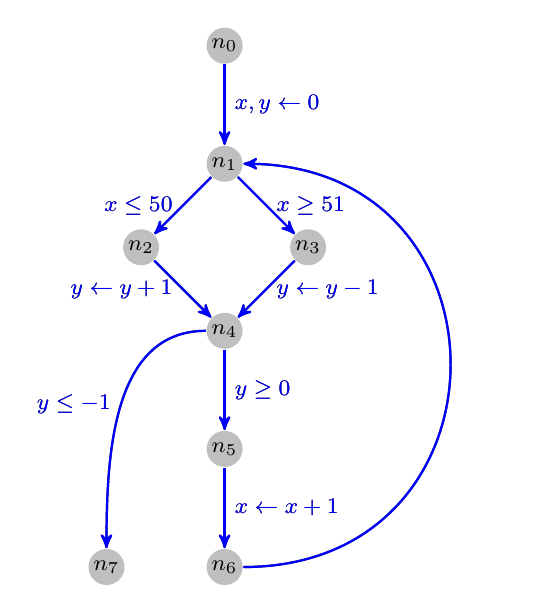
\begin{tikzpicture}[->,>=stealth',auto,node distance=1.5cm,
                    semithick,font=\footnotesize]

	\node[state] (n0) {$n_0$};
	\node[state] (n1) [below of=n0] {$n_1$};
	\node[state] (n2) [below left of=n1] {$n_2$};
	\node[state] (n3) [below right of=n1] {$n_3$};
	\node[state] (n4) [below left of=n3] {$n_4$};
	\node[state] (n5) [below of=n4] {$n_5$};
	\node[state] (n6) [below of=n5] {$n_6$};
	\node[state] (n7) [left of=n6] {$n_7$};

	\node (n8) [right of=n6] {};
	\node (n9) [right of=n1] {};

  \path<-1> [transition] 
		(n0) edge              node {$x,y \leftarrow 0$} (n1);
  \path<-2> [transition] 
        (n1) edge			   node [left] {$x \leq 50$} (n2);
  \path<-9> [transition] 
        (n1)  edge              node [right] {$x \geq 51$} (n3);
  \path<-3> [transition] 
        (n2) edge              node [left] {$y \leftarrow y+1$} (n4);
  \path<-10> [transition] 
        (n3) edge			   node [right] {$y \leftarrow y-1$} (n4);
  \path<-4> [transition] 
        (n4) edge			   node {$y \geq 0$} (n5);
  \path<-12> [transition] 
		(n4) edge  [out = 180, in=90] node [left] {$y \leq -1$} (n7);
  \path<-5> [transition] 
        (n5) edge              node {$x \leftarrow x+1$} (n6);
  \path<-6> [transition] 
        (n6) edge [out=0, in=0, distance=3.5cm] node {} (n1);

  \path<2-> [transition2] 
		(n0) edge              node {$x,y \leftarrow 0$} (n1);
  \path<3-> [transition2] 
        (n1) edge			   node [left] {$x \leq 50$} (n2);
  \path<10-> [transition2] 
        (n1)  edge              node [right] {$x \geq 51$} (n3);
  \path<4-> [transition2] 
        (n2) edge              node [left] {$y \leftarrow y+1$} (n4);
  \path<11-> [transition2] 
        (n3) edge			   node [right] {$y \leftarrow y-1$} (n4);
  \path<5-> [transition2] 
        (n4) edge			   node {$y \geq 0$} (n5);
  \path<13-> [transition2] 
		(n4) edge  [out = 180, in=90] node [left] {$y \leq -1$} (n7);
  \path<6-> [transition2] 
        (n5) edge              node {$x \leftarrow x+1$} (n6);
  \path<7-> [transition2] 
        (n6) edge [out=0, in=0, distance=3.5cm] node {} (n1);
\end{tikzpicture}
\end{column}
\begin{column}{5cm}
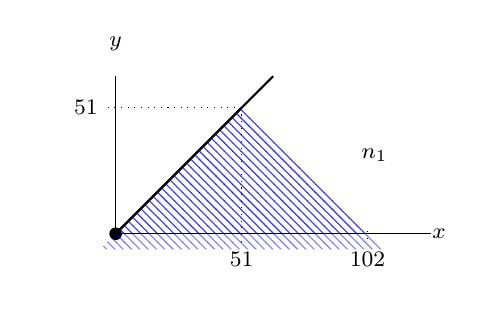
\begin{tikzpicture}[y=.2cm, x=.2cm,font=\footnotesize]

	\node (t1) at (-5,-4) {};
	\node (t2) at (13,11) {};
	\fill<2-6>[line] (0,0) circle (0.4);
	\draw<7-8>[line] (0,0) -- (10,10) -- cycle;
	\draw<9->[line] (0,0) -- (8,8) -- cycle;
	
	\fill<12-13>[polyhedra] (-1,-1) -- (8,8) -- (17,-1) -- cycle;
	\fill<14->[polyhedra] (0,0) -- (8,8) -- (16,0) -- cycle;
	
	%\draw<10-11>[line] (-1,-1) -- (10,10) -- cycle;
	%\fill<10-11>[polyhedra] (-1,-1) -- (10,10) -- (13,10) -- (13,-1) -- (0,-1) -- cycle;
	%\fill<12-13>[polyhedra] (0,0) -- (10,10) -- (13,10) -- (13,0) -- cycle;
	%\draw<12-13>[line] (0,0) -- (10,10) -- cycle;

 	%axis
	\draw (0,0) -- coordinate (x axis mid) (20,0);
    \draw (0,0) -- coordinate (y axis mid) (0,10);

	%ticks and labels      
     		\draw<9-> [dotted](8,8) -- (-3pt,8) 
     			node[anchor=east] {$51$}; 
     		\draw<9-> [dotted] (8,8) -- (8,-3pt) 
     			node[anchor=north] {$51$}; 
     		\draw<12-> [dotted] (16,1pt) -- (16,-3pt) 
     			node[anchor=north] {$102$}; 

	\node[right=1.9cm] at (x axis mid) {$x$};
	\node[above=1.2cm] at (y axis mid) {$y$};

	\node[right=3cm] at (y axis mid) {$n_1$};
\end{tikzpicture} 
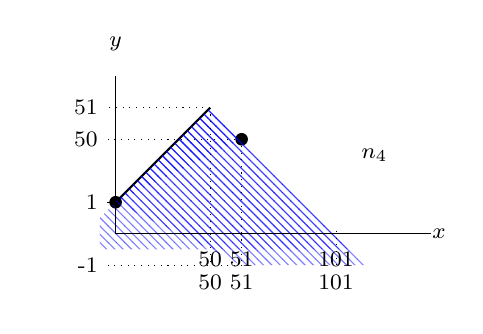
\begin{tikzpicture}[y=.2cm, x=.2cm,font=\footnotesize]

	\node (t1) at (-5,-4) {};
	\node (t2) at (13,11) {};
	\fill<4-7>[line] (0,2) circle (0.4);
	\draw<8->[line] (0,2) -- (6,8);
	
	\fill<11-12>[circle] (8,6) circle (0.4);
	\fill<11-12>[polyhedra] (8,6) -- (6,8) -- (0,2) -- cycle;

	\fill<13-14>[polyhedra] (6,8) -- (15,-1) -- (-1,-1) -- (-1,1) -- (0,2) -- cycle;
	\fill<15->[polyhedra] (6,8) -- (16,-2) -- (8,-2) -- (0,2) -- cycle;
	%\draw<11-12>[line] (-2,0) -- (8,10);
	%\fill<11-12>[polyhedra] (-2,-1) -- (-2,0) -- (8,10) -- (13,10) -- (13,-1) --
	% cycle;
	%\fill<11-12>[polyhedra] (-2,-1) -- (-2,0) -- (6,8) -- (6,-1) -- cycle;
	%\fill<11-13>[polyhedra] (8,6) -- (12,10) -- (13,10) -- (13,-1) -- (8,-1) -- cycle;

	%\draw<13-13>[line] (0,2) -- (8,10);
	%\draw<13-13>[line] (0,2) -- (8,-1);
	%\fill<13-13>[polyhedra] (0,2) -- (8,10) -- (13,10) -- (13,-1) -- (8,-1) -- cycle;
	%\fill<13-13>[polyhedra] (0,2) -- (6,8) -- (6,2) --  cycle;

 	%axis
	\draw (0,0) -- coordinate (x axis mid) (20,0);
    \draw (0,0) -- coordinate (y axis mid) (0,10);

	%labels      
	\node[right=1.9cm] at (x axis mid) {$x$};
	\node[above=1.2cm] at (y axis mid) {$y$};

	\node[right=3cm] at (y axis mid) {$n_4$};
	%ticks
     		\draw<4-> (1pt,2) -- (-3pt,2) 
     			node[anchor=east] {1}; 
     		\draw<15-> [dotted] (8,-2) -- (-3pt,-2) 
     			node[anchor=east] {-1}; 
     		\draw<8-> [dotted](6,8) -- (-3pt,8) 
     			node[anchor=east] {$51$}; 
     		\draw<8-14> [dotted] (6,8) -- (6,-3pt) 
     			node[anchor=north] {$50$}; 
     		\draw<15-> [dotted] (6,8) -- (6,-2) 
     			node[anchor=north] {$50$}; 
     		\draw<11-12> [dotted] (8,6) -- (-3pt,6) 
     			node[anchor=east] {$50$}; 
     		\draw<11-12> [dotted](8,6) -- (8,-3pt) 
     			node[anchor=north] {$51$}; 
     		\draw<15-> [dotted](8,0) -- (8,-2) 
     			node[anchor=north] {$51$}; 
     		\draw<13-14> [dotted] (14,1pt) -- (14,-3pt) 
     			node[anchor=north] {$101$}; 
     		\draw<15-> [dotted] (14,1pt) -- (14,-2) 
     			node[anchor=north] {$101$}; 
     		%\draw (2,1pt) -- (2,-3pt) 
     		%	node[anchor=north] {1}; 

\end{tikzpicture} 
\only<1-8>{Ascending iterations}
\only<10-13>{Ascending iterations}
\only<9>{Descending iterations}
\only<14->{Descending iterations}
\end{column}
\end{columns}
\end{frame}

\section[Path focusing]{Using SMT-solving to focus new paths}

\begin{frame}
  \frametitle{Principle}

D. Monniaux \& L. Gonnord
\bigskip
\begin{itemize}
\item Compute the fixpoint iterations on a multigraph
\item Take a set $P_R$ of nodes
\item Distinguish all the paths between 2 nodes of $P_R$
\end{itemize}
\bigskip
\visible<2>{
Exponential number of paths:
\begin{itemize}
\item We don't construct this graph explicitly
\item We use SMT-solving to find interesting paths
\end{itemize}
}
\end{frame}

\begin{frame}
  \frametitle{Reducing the graph}

\begin{columns}
\begin{column}{5.5cm}
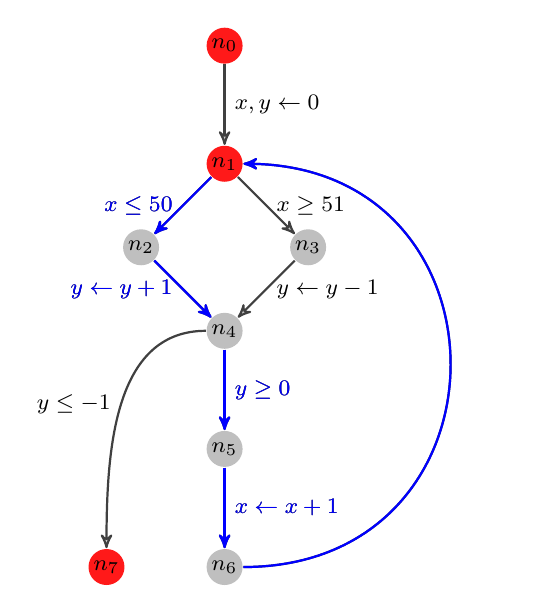
\begin{tikzpicture}[->,>=stealth',auto,node distance=1.5cm,
                    semithick,font=\footnotesize]

	\node[PRstate] (n0) {$n_0$};
	\node[PRstate] (n1) [below of=n0] {$n_1$};
	\node[state] (n2) [below left of=n1] {$n_2$};
	\node[state] (n3) [below right of=n1] {$n_3$};
	\node[state] (n4) [below left of=n3] {$n_4$};
	\node[state] (n5) [below of=n4] {$n_5$};
	\node[state] (n6) [below of=n5] {$n_6$};
	\node[PRstate] (n7) [left of=n6] {$n_7$};


  \path [transition] 
		(n0) edge              node {$x,y \leftarrow 0$} (n1);
  \path<-2> [transition] 
        (n1) edge			   node [left] {$x \leq 50$} (n2);
  \path [transition] 
        (n1)  edge              node [right] {$x \geq 51$} (n3);
  \path<-2> [transition] 
        (n2) edge              node [left] {$y \leftarrow y+1$} (n4);
  \path [transition] 
        (n3) edge			   node [right] {$y \leftarrow y-1$} (n4);
  \path<-2> [transition] 
        (n4) edge			   node {$y \geq 0$} (n5);
  \path [transition] 
		(n4) edge  [out = 180, in=90] node [left] {$y \leq -1$} (n7);
  \path<-2> [transition] 
        (n5) edge              node {$x \leftarrow x+1$} (n6);
  \path<-2> [transition] 
        (n6) edge [out=0, in=0, distance=3.5cm] node {} (n1);


  \path<3-> [transition2] 
        (n1) edge			   node [left] {$x \leq 50$} (n2);
  \path<3-> [transition2] 
        (n2) edge              node [left] {$y \leftarrow y+1$} (n4);
  \path<3-> [transition2] 
        (n4) edge			   node {$y \geq 0$} (n5);
  \path<3-> [transition2] 
        (n5) edge              node {$x \leftarrow x+1$} (n6);
  \path<3-> [transition2] 
        (n6) edge [out=0, in=0, distance=3.5cm] node {} (n1);
\end{tikzpicture}
\end{column}
\begin{column}{5.5cm}
\visible<2->{
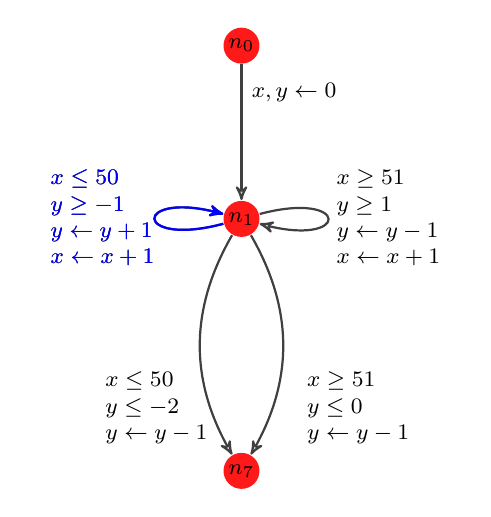
\begin{tikzpicture}[->,>=stealth',auto,node distance=3.2cm,
                    semithick,font=\footnotesize]

	\node[PRstate] (n0) {$n_0$};
	\node[PRstate] (n1) [below of=n0,yshift=1cm] {$n_1$};
	\node[PRstate] (n7) [below of=n1] {$n_7$};


  \path [transition] 
		(n0) edge              node [yshift=5mm] {$x,y \leftarrow 0$} (n1);
  \path [transition] 
		(n1) edge    [bend left]  node [right,yshift=-0.8cm]  {$
		\begin{array}{l}
			x \geq 51 \\
			y \leq 0 \\
			y \leftarrow y-1
		\end{array}
		$} (n7);
  \path [transition] 
		(n1) edge    [bend right]  node [left,yshift=-0.8cm,xshift=4mm] {$
		\begin{array}{l}
			x \leq 50 \\
			y \leq -2 \\
			y \leftarrow y-1
		\end{array}
		$} (n7);
  \path<-2> [transition] 
		(n1) edge    [loop left,distance=1.2cm]  node [left,xshift=3mm] {$
		\begin{array}{l}
			x \leq 50 \\
			y \geq -1 \\
			y \leftarrow y+1 \\
			x \leftarrow x+1 
		\end{array}
		$} (n1);
  \path<3-> [transition2] 
		(n1) edge    [loop left,distance=1.2cm]  node [left,xshift=3mm] {$
		\begin{array}{l}
			x \leq 50 \\
			y \geq -1 \\
			y \leftarrow y+1 \\
			x \leftarrow x+1 
		\end{array}
		$} (n1);
  \path [transition] 
		(n1) edge    [loop right,distance=1.2cm]  node [right,xshift=-2mm] {$
		\begin{array}{l}
			x \geq 51 \\
			y \geq 1 \\
			y \leftarrow y-1 \\
			x \leftarrow x+1 
		\end{array}
		$} (n1);
  %\path [transition] 
  %      (n6) edge [out=0, in=0, distance=3.5cm] node {} (n1);
\end{tikzpicture}
}
\end{column}
\end{columns}
\end{frame}

\begin{frame}
  \frametitle{using SMT-solving to find new paths}
\begin{itemize}
\item Compute an SMT formula $\rho$ expressing the semantic of the program
\item $\rho$ contains reachability predicates
\end{itemize}
\bigskip
To find a path from $p_1$ to $p_2$, ($p_1,p_2 \in P_R$) :
$$\rho  \wedge b_{p_1} \wedge x_1 \in X_{p_1} \wedge \bigvee_{p_2 \in succ(p_1)}
 (b_{p_2} \wedge x_2 \notin X_{p_2})$$

\footnotesize{
$b_{p_i}$: reachability predicate for $p_i$

$X_{p_i}$: abstract domain of node $p_i$
}
\end{frame}

\begin{frame}[containsverbatim]
	\frametitle{Example}
\begin{center}
\begin{lstlisting}
	int x = 0;
	int d = 1;
	
	while (true) {
		if (x == 0) d=1;
		if (x == 1000) d=-1;
		x +=d;
	}
\end{lstlisting}
\end{center}
\begin{itemize}
\item $x$ incremented until it is equal to $1000$,
\item $x$ decremented until it is equal to $0$,
\item restart\ldots
\end{itemize}

\end{frame}

\begin{frame}
  \frametitle{Example}
\begin{columns}
\begin{column}{7cm}
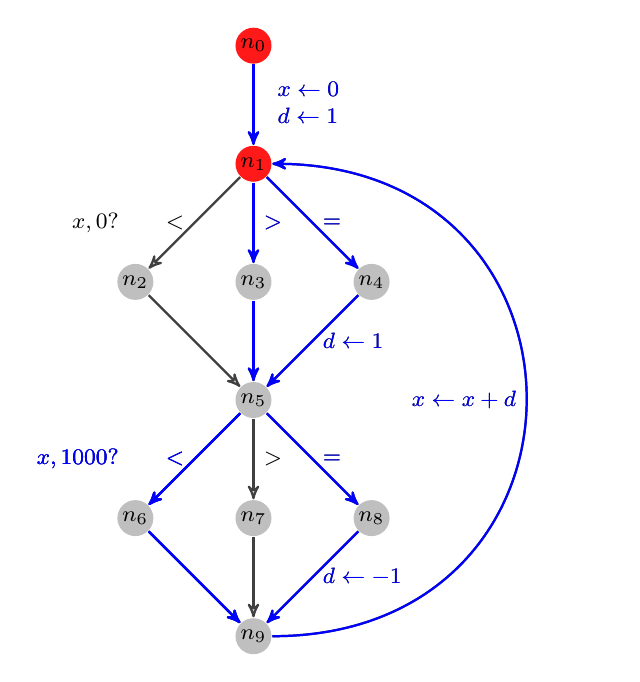
\begin{tikzpicture}[->,>=stealth',auto,node distance=1.5cm,
                    semithick,font=\footnotesize]
	\node[PRstate] (n0) {$n_0$};
	\node[PRstate] (n1) [below of=n0] {$n_1$};
	\node[state] (n3) [below of=n1] {$n_3$};
	\node[state] (n2) [left of=n3] {$n_2$};
	\node[state] (n4) [right of=n3] {$n_4$};
	\node[state] (n5) [below of=n3] {$n_5$};
	\node[state] (n7) [below of=n5] {$n_7$};
	\node[state] (n6) [left of=n7] {$n_6$};
	\node[state] (n8) [right of=n7] {$n_8$};
	\node[state] (n9) [below of=n7] {$n_9$};

  \path [transition] 
		(n0) edge              node  {$\begin{array}{l}
		x \leftarrow 0 \\
		d \leftarrow 1 
		\end{array}$} (n1);
  \path [transition] 
        (n1) edge			   node [left] {$x,0?$~ ~ ~ $<$} (n2);
  \path [transition] 
        (n1)  edge              node {$>$} (n3);
  \path [transition] 
        (n1)  edge              node [right] {$=$} (n4);
  \path [transition] 
        (n3) edge              node  {} (n5);
  \path [transition] 
        (n2) edge			   node {} (n5);
  \path [transition] 
        (n4) edge			   node [right] {$d \leftarrow 1$} (n5);
  \path [transition] 
        (n5) edge			   node [left] {$x,1000?$ ~ ~ ~$<$} (n6);
  \path [transition] 
        (n5) edge			   node {$>$} (n7);
  \path [transition] 
        (n5) edge			   node [right] {$=$} (n8);
  \path [transition] 
        (n6) edge              node {} (n9);
  \path [transition] 
        (n7) edge              node {} (n9);
  \path [transition] 
        (n8) edge              node [right] {$d \leftarrow -1$} (n9);
  \path [transition] 
        (n9) edge [out=0, in=0, distance=4.3cm] node [left] {$x \leftarrow x+d$} (n1);

  \path<1> [transition2] 
		(n0) edge              node  {$\begin{array}{l}
		x \leftarrow 0 \\
		d \leftarrow 1 
		\end{array}$} (n1);

  \path<2-3> [transition2] 
        (n1)  edge              node [right] {$=$} (n4);
  \path<2-3> [transition2] 
        (n4) edge			   node [right] {$d \leftarrow 1$} (n5);
  \path<2-5> [transition2] 
        (n5) edge			   node [left] {$x,1000?$ ~ ~ ~$<$} (n6);
  \path<2-5> [transition2] 
        (n6) edge              node {} (n9);
  \path<2-> [transition2] 
        (n9) edge [out=0, in=0, distance=4.3cm] node [left] {$x \leftarrow x+d$} (n1);
  \path<4-8> [transition2] 
        (n1) edge			   node {$>$} (n3);
  \path<4-8> [transition2] 
        (n3) edge			   node {} (n5);
	
  \path<6-7> [transition2] 
        (n5) edge			   node [right] {$=$} (n8);
  \path<6-7> [transition2] 
        (n8) edge              node [right] {$d \leftarrow -1$} (n9);
  \path<8> [transition2] 
        (n5) edge			   node [left] {$x,1000?$ ~ ~ ~$<$} (n6);
  \path<8> [transition2] 
        (n6) edge              node {} (n9);
\end{tikzpicture}
\end{column}
\begin{column}{5cm}
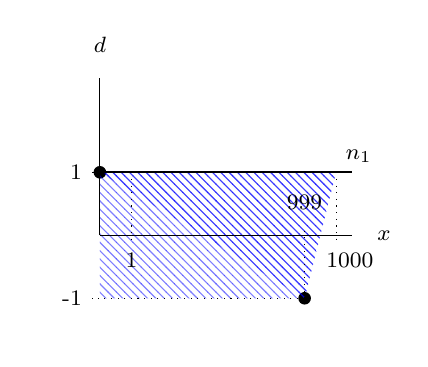
\begin{tikzpicture}[y=.2cm, x=.2cm,font=\footnotesize]

	\fill<-1>[line] (0,4) circle (0.4);
	\fill<6-8>[line] (13,-4) circle (0.4);
	\fill<7>[polyhedra] (13,-4) -- (0,4) -- (15,4) -- cycle;
	\fill<8>[polyhedra] (13,-4) -- (0,-4) -- (0,4) -- (15,4) -- cycle;
	\draw<3>[line] (0,4) -- (2,4) -- cycle;
	\draw<2>[line] (0,4) -- (16,4) -- cycle;
	\draw<4>[line] (0,4) -- (16,4) -- cycle;
	\draw<5->[line] (0,4) -- (15,4) -- cycle;

 	%axis
	\draw (0,0) -- coordinate (x axis mid) (16,0);
    \draw (0,0) -- coordinate (y axis mid) (0,10);

	%ticks and labels      
	\node[right=1.8cm] at (x axis mid) {$x$};
	\node[above=1.2cm] at (y axis mid) {$d$};
	
	\node at (-4,-6) {};

     		\draw<1-> (1pt,4) -- (-3pt,4) 
     			node[anchor=east] {1}; 
     		\draw<6-> [dotted] (13,-4) -- (-3pt,-4) 
     			node[anchor=east] {-1}; 
     		\draw<3-3> [dotted] (2,4) -- (2,-3pt) 
     			node[anchor=north] {1}; 
     		\draw<5-> [dotted] (15,4) -- (15,-3pt) 
     			node[anchor=north,xshift=5pt] {1000}; 
     		\draw<6-> [dotted] (13,-4) -- (13,3pt) 
     			node[anchor=north,yshift=15pt] {999}; 

	\node[right=3cm] at (y axis mid) {$n_1$};
\end{tikzpicture} 
\end{column}
\end{columns}
\end{frame}

\begin{frame}
\frametitle{Other Applications}

\begin{itemize}
\item Analysis with pointers
\item Overflows analysis
\item \ldots
\end{itemize}

\end{frame}

\section[Work in progress]{Work in progress}

\begin{frame}
  \frametitle{What is done}
\begin{itemize}
\item a small analyzer, using LLVM and Apron
\item implementation of the Lookahead widening technique
\item some tests
\end{itemize}
\end{frame}

\begin{frame}
  \frametitle{Work in progress / Future work}
\begin{itemize}
\item implementation of the Path-focusing technique
\item experimental evaluation
\item find and correct shortcomings of the method
\item Some questions :
\begin{itemize}
\item  How to determine the best $P_R$ ?
\end{itemize}
\end{itemize}
\end{frame}

\begin{frame}
\begin{center}
Thank you!
\end{center}
\end{frame}

\end{document}

%%% Local Variables:
%%% mode: latex
%%% TeX-master: t
%%% ispell-local-dictionary: "american"
%%% End:
